\subsection{Study of Neutrino Freeze-out using  the Boltzmann-Einstein Equation}\label{ch:param_studies}
In this section we remove the instantaneous freeze-out assumption  and present a more precise study of  neutrino freeze-out, i.e., we do not assume that the distribution is either in chemical or kinetic equilibrium or is free-streaming.
The required mathematical theory and numerical method is developed in Appendices \ref{ch:vol_forms}, \ref{ch:boltz_orthopoly}, and \ref{ch:coll_simp}.  Here we focus on the physical implications, in particular the dependence of the freeze-out process on natural constants. This allows us identify potential avenues by which the tension between observed and theoretical values of $N^{\mathrm{eff}}_\nu$ may be alleviated.   Our study also constrains the time and/or temperature variation of certain natural constants by comparing the results with measurements of $N_\nu^{\mathrm{eff}}$. Further details on this work can be found in \cite{Birrell:2014uka}. The topic of time variation of natural constants is a very active field with a long history; for a comprehensive review of this area, with which we make only slight contact,  see \cite{Uzan:2010pm}.  







\subsubsection{Neutrino Freeze-Out Temperature and Relaxation Time} 
To connect with the instantaneous freeze-out model from Section \ref{ch:model_ind}, we now give a definition of the kinetic freeze-out temperature that is applicable to the Boltzmann-Einstein equation model and use this to calculate the neutrino freeze-out temperature. Any such definition will be only approximate, as the freeze-out process is not a sharp transition.  Our definition is motivated in part the treatment in \cite{Kolb:1990vq}. 

We first define a characteristic length between scatterings. Using the formula \req{n_div}, we obtain the fractional rate of change of comoving particle number
\begin{align}
\frac{\frac{d}{dt}(a^3 n)}{a^3n}=\frac{g_\nu}{2\pi^2n}\int C[f]p^2/Edp\,.
\end{align}
Here we don't want the net change, but rather to count the number of interactions.  For that reason, we imagine that only one direction of the process is operational and define the relaxation rate\index{relaxation rate}
\begin{align}
\Gamma\equiv\frac{g_\nu}{2\pi^2n}T^2\int \tilde C[f]zdz\,,
\end{align}
where the one way collision is $\tilde C[f]$ is computed as in \req{coll} except with $F$ replaced by 
\begin{equation}
\tilde F=f_1(p_1)f_2(p_2)f^3(p_3)f^4(p_4)\,.
\end{equation}
If particle type $1$ also participates in the reverse of the reaction $1+2\rightarrow 3+4$ then a corresponding term for the reverse reaction must also be added.  The key difference is there is no minus sign; here we are counting reactions, not net particle number change.

Using the average velocity, which for (effectively massless) neutrinos is $\bar v=c=1$, we obtain what we call the scattering length\index{scattering length}
\begin{align}
L_\Gamma&\equiv\frac{\bar v}{\Gamma}=\frac{\int_0^\infty\frac{1}{\Upsilon^{-1}e^z+1}z^2dz}{\int_0^\infty \tilde C[f] z^2/E dz}\,.
\end{align}
This can be compared to the Hubble length $L_H=c/H$\index{Hubble length} and the temperature at which $L_\Gamma=L_H$ we call the freeze-out temperature\index{freeze-out temperature} for that reaction.  Figure \ref{fig:scatt_length} shows the scattering length and $L_H$ for various types of neutrino reactions.  The solid line corresponds to the annihilation process $e^+e^-\rightarrow \nu\bar\nu$, the dashed line corresponds to the scattering $\nu e^\pm\rightarrow \nu e^\pm$, and the dot-dashed line corresponds to the combination of all processes involving only neutrinos.  The freeze-out temperatures in MeV are given in Table \ref{table:freeze-out_temp}.

\begin{table}[ht]
\centering 
\begin{tabular}{|c|c|c|c|}
\hline
              & $e^+e^-\rightarrow \nu\bar\nu$ & $\nu e^\pm\rightarrow \nu e^\pm$ & $\nu$-only processes\\
\hline
$\nu_e$ &2.29 & 1.15&0.910\\
\hline
$\nu_{\mu,\tau}$ &3.83 & 1.78& 0.903\\
\hline
\end{tabular}
\caption{Freeze-out temperatures in MeV for electron neutrinos and for $\mu$,$\tau$ neutrinos.}
\label{table:freeze-out_temp}
\end{table}

%%%%%%%%%%%%%%%%%%%%%%%%%%%%%%%%%%%%%%%
\begin{figure}[ht]
\centerline{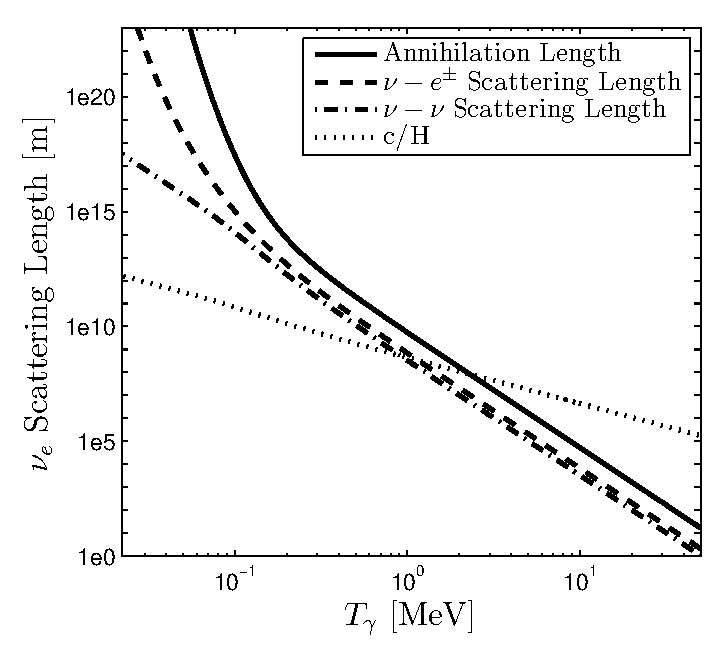
\includegraphics[height=6cm]{04-birrell/ParametricStudies/Figures/nu_e_scattering_length_eta_0_23.eps}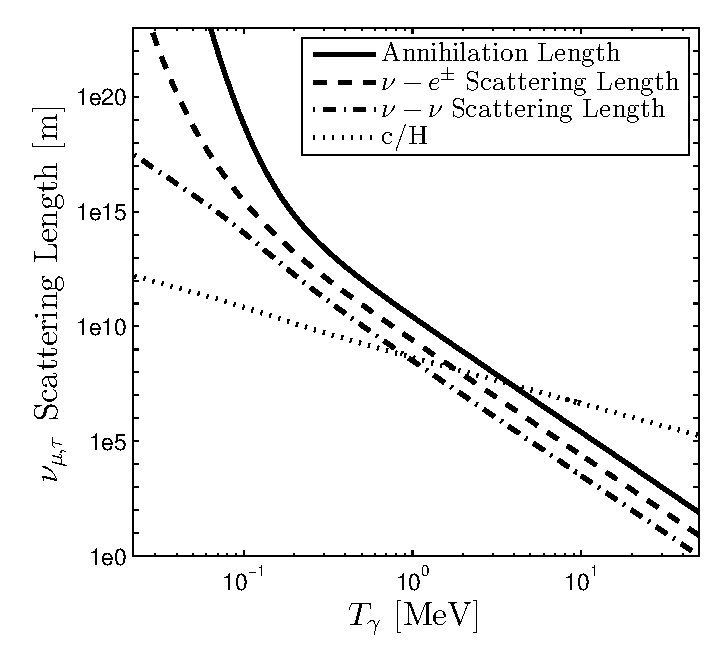
\includegraphics[height=6cm]{04-birrell/ParametricStudies/Figures/nu_mu_scattering_length_eta_0_23.eps}}
\caption{\cccite{Birrell:2014uka}. Comparison of Hubble parameter to neutrino scattering length for various types of SM processes.  }\label{fig:scatt_length}
\end{figure}
%%%%%%%%%%%%%%%%%%%%%%%%%%%%%%%%%%%%%%%


We now consider the the relaxation time\index{relaxation time} for a given reaction, defined by $\tau=1/\Gamma$.  Suppose we have a time interval $t_f>t_i$  and corresponding temperature interval $T_f<T_i$ during which there is no reheating and the Universe is radiation dominated.  Normalizing time so $t=0$ corresponds to the temperature $T_i$ we have
\begin{equation}\label{ch6:H_eq}
\dot a/a=-\dot T/T\,,\hspace{2mm} H=\frac{C}{2Ct+T_i^2}\propto T^2
\end{equation}
where $C$ is a constant that depends on the energy density and the Planck mass.  Its precise form will not be significant for us.  Note that \req{ch6:H_eq} implies
\begin{equation}
1/H(t)-1/H(0)=2t\,.
\end{equation}

At $T\gg m_e$, the rates for reactions under consideration from Tables \ref{table:nu_e_reac} and \ref{table:nu_mu_reac} scale as $\Gamma\propto T^5$.  Therefore, supposing $H(T_f)/\Gamma(T_f)=1$ (which occurs at $T_f=O(1\MeV)$ as seen in the above figures), at any time $t_f>t>t_i$ we find 
\begin{align}\label{relax_time}
\tau(t)/t=&\frac{2}{\Gamma(t)}\left(\frac{1}{H(t)}-\frac{1}{H(0)}\right)^{-1}=\frac{2T_f^5}{\Gamma(T_f)T^5}\left(\frac{T_f^2}{H(T_f)T^2}-\frac{T_f^2}{H(T_f)T_i^2}\right)^{-1}\\
=&\frac{2T_f^3}{T^3}\left(1-\frac{T^2}{T_i^2}\right)^{-1}\,.
\end{align}
Therefore, given any time $t_i<t_0<t_f$ we have
\begin{equation}\label{ch6:tau_eq}
\tau(t)<\tau(t_0)=\frac{2T_f^3}{T_0^3}\left(1-\frac{T_0^2}{T_i^2}\right)^{-1}\Delta t \text{ \,for all } t<t_0\,,
\end{equation}
where $\Delta t=t_0-t_i=t_0$.

 The first reheating period that precedes neutrino freeze-out is the disappearance of muons and pions around $O(100\MeV)$, as seen in Figure \ref{fig:energy_frac}, and so we let $T_i=100\MeV$. \req{ch6:tau_eq} is minimized at $T_0\approx 77.5\MeV$ at which point we have 
\begin{equation}
\tau(t)<10^{-5} \Delta t_0 \text{ for } t<t_0.
\end{equation}
This shows that the relaxation time during the period between $100\MeV$ and $77.5\MeV$ is at least five orders of magnitude smaller than the corresponding time interval.  Therefore the system has sufficient time to relax back to equilibrium after any potential non-equilibrium aspects developed during the reheating period.  Thus justifies our assumption that the neutrino distribution has the equilibrium Fermi Dirac form at $T=O(10 \MeV)$ when we begin our numerical simulation. This can also be demonstrated numerically in Figure \ref{fig:relax}, where we have initialized the system at $T_\gamma=12\MeV$ with a non-equilibrium distribution of $\mu$ and $\tau$ neutrinos, giving them $\Upsilon=0.9$, and let them evolve under the Boltzmann-Einstein equation.  We see that after approximately $10^{-3}$ seconds the system relaxes back to equilibrium, well before neutrino freeze-out near $t=1$s.

%%%%%%%%%%%%%%%%%%%%%%%%%%%%%%%%%%%%%%%
\begin{figure} 
%04-birrell/ParametricStudies/Figures/
\begin{minipage}{\linewidth}
\makebox[0.48\linewidth]%
{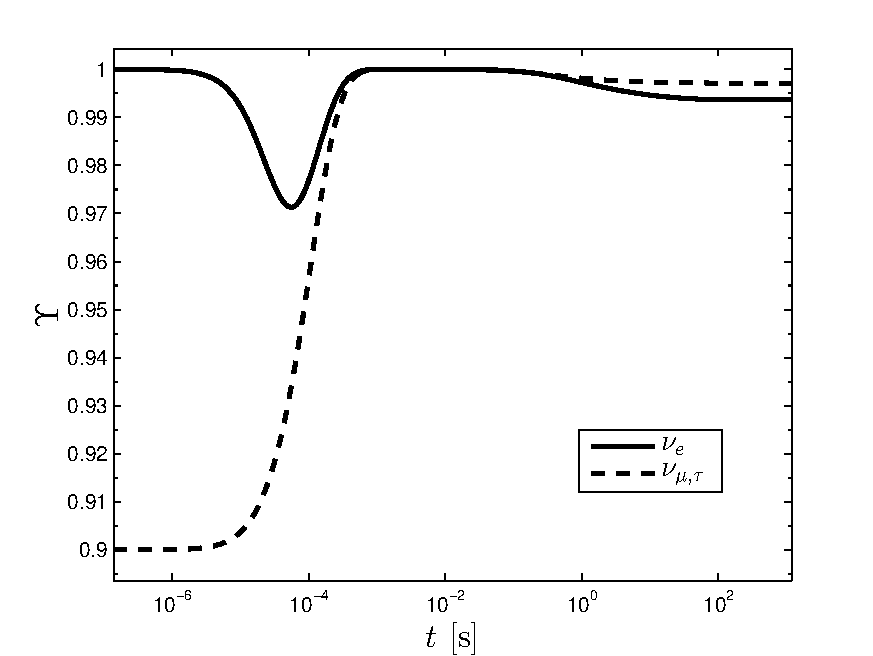
\includegraphics[height=5.5cm]{04-birrell/ParametricStudies/Figures/Ups_relax.eps}}
\makebox[0.48\linewidth]%
{\hspace{6mm}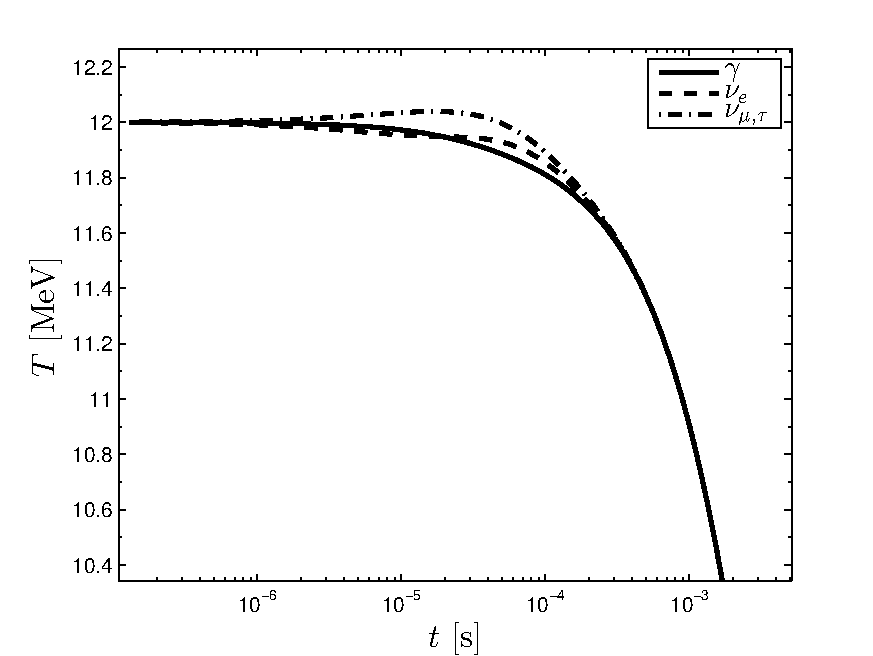
\includegraphics[height=5.5cm]{04-birrell/ParametricStudies/Figures/T_relax.eps}}
\end{minipage}
\caption{Starting at $12\MeV$, this figure shows the relaxation of a non-equilibrium $\mu,\tau$-neutrino distribution towards equilibrium. The fugacities are shown in the left frame while the temperatures are shown in the right frame.\label{fig:relax}}
 \end{figure}
%%%%%%%%%%%%%%%%%%%%%%%%%%%%%%%%%%%%%%%







\subsubsection{Dependence of effective neutrino number on SM parameters}\label{sec:param_char}

Next we identify the key SM parameters that influence the effective number of neutrinos and study the effect that  their variation has on $N_\nu^{\mathrm{eff}}$.


\paragraph{Weinberg Angle}

The Weinberg angle\index{Weinberg angle} is one of the key standard model parameters that impacts the neutrino freeze-out process.  More specifically, it is found in the matrix elements of weak force processes, including the reactions $e^+e^-\rightarrow \nu\bar\nu$ and $\nu e^\pm\rightarrow \nu e^\pm$ as found in Tables \ref{table:nu_e_reac} and \ref{table:nu_mu_reac}.  It is determined by the $SU(2)\times U(1)$ coupling constants $g$, $g^{'}$  by
\begin{equation}
\sin(\theta_W)=\frac{g^{'}}{\sqrt{g^2+(g^{'})^2}}\,.
\end{equation}
It is also related to the mass of the $W$ and $Z$ bosons and the Higgs vacuum expectation value $v$ by
\begin{equation}
M_Z=\frac{1}{2}\sqrt{g^2+(g^{'})^2}v\,,\hspace{2mm}  M_W=\frac{1}{2}gv\,,\hspace{2mm} \cos(\theta_W)=\frac{M_W}{M_Z}\,,
\end{equation}
as well as the electromagnetic coupling strength
\begin{equation}
e=2M_W\sin(\theta_W)/v=\frac{gg^{'}}{\sqrt{g^2+(g^{'})^2}}\,.
\end{equation}
It has a measured value in vacuum $\theta_W\approx 30^\circ$, giving $\sin(\theta_W)\approx 1/2$, but its value is not fixed within the Standard Model. For this reason, a time or temperature variation can be envisioned and this would have an observable impact on the neutrino freeze-out process, as measured by $N_\nu^{\mathrm{eff}}$.

In letting $\sin(\theta_W)$, and hence $g$ and $g^{'}$, vary we must fix the electromagnetic coupling $e$ so as not to impact sensitive cosmological observables such as Big Bang Nucleosynthesis.  Fixing $v$, the smallest $M_W$ can become is when $\sin(\theta_W)=1$, yielding a reduction in $M_W$ by a factor of $2$.  This implies that $M_Z>M_W\gg |p|$ for neutrino momentum $p$ in the energy range of neutrino freeze-out, around $1\MeV$, even as we vary $\sin(\theta_W)$.  This approximation is inherent in the formulas for the matrix elements  in Tables  \ref{table:nu_e_reac} and \ref{table:nu_mu_reac} and continues to be valid here. We will characterize the dependence of $N_\nu^{\mathrm{eff}}$ on $\sin(\theta_W)$ in Section \ref{sec:param_char} below, but first we identify the remaining parameter dependence in the Boltzmann-Einstein system


\paragraph{Interaction Strength} Beyond the Weinberg angle, the remaining  dependence of the Boltzmann-Einstein system on dimensioned quantities during  neutrino freeze-out  can be combined in an overall interaction strength factor.   To show this, we now convert the system  to dimensionless form. Letting $m_e$ be the mass scale and $M_p/m_e^2$ be the time scale the Einstein equations take the form
\begin{equation}
H^2=\frac{\rho}{3}\,,\hspace{2mm}\dot\rho=-3H(\rho+P)\,.
\end{equation}
 Since $e^\pm$ are the only (effectively) massive particles in the system, by scaling all energies, momenta, energy densities, pressures, and temperatures by $m_e$ we have removed all scale dependent parameters from the Einstein equations.  The Boltzmann-Einstein equation becomes
\begin{equation}\label{eta_def}
\partial_tf-pH\partial_pf=\eta\frac{C[f]}{E}\,,\hspace{2mm}\eta\equiv M_p m_e^3G_F^2\,,
\end{equation}
where we have also factored out of $C[f]$ the $G_F^2$ term that is common to all of the neutrino interaction matrix elements. 

Aside from the $\theta_W$ dependence of the matrix elements seen in Tables \ref{table:nu_e_reac} and \ref{table:nu_mu_reac}, the complete dependence on natural constants  is now contained in a single dimensionless neutrino interaction strength parameter\index{neutrino interaction strength} $\eta$ with the vacuum present day value,
\begin{equation}\label{eta0_def}
\eta_0\equiv \left.M_p m_e^3 G_F^2\right|_0  \approx 0.04421\, .
\end{equation}



\paragraph{QED Corrections to Equation of State}\label{app:QED_corr} 
At the time of neutrino freeze-out, the universe is at sufficiently high temperature for photons and $e^\pm$ to be in chemical and kinetic equilibrium.  The temperature is also sufficiently high for QED corrections to the photon and $e^\pm$ equation of state to be non-negligible.  Therefore, in our study here we use the results given in \cite{Heckler:1994tv,Mangano:2001iu} to include these in our computation by modifying the combined photon, $e^\pm$ equation of state
\begin{align}
P=P^0+P^{int},\hspace{2mm} \rho=-P+T\frac{dP}{dT}\,,
\end{align}
where
\begin{align}
P^{int}=&-\frac{1}{2\pi^2}\int_0^\infty\left[\frac{k^2}{E_k}\frac{\delta m_e^2}{e^{E_k/T}+1}+\frac{k}{2}\frac{\delta m_\gamma^2}{e^{k/T}-1}\right]dk\,,\hspace{2mm} E_k=\sqrt{k^2+m_e^2}\,,\\
\delta m_e^2=&\frac{2\pi\alpha^2}{3}+\frac{4\alpha}{\pi}\int_0^\infty \frac{k^2}{E_k}\frac{1}{e^{E_k/T}+1}dk\,,\hspace{2mm} \delta m_\gamma^2=\frac{8\alpha}{\pi}\int_0^\infty \frac{k^2}{E_k}\frac{1}{e^{E_k/T}+1}dk\,,
\end{align}
and $P^0$ is the pressure of a non-interacting gas of photons and $e^\pm$ in chemical equilibrium.


\paragraph{Dependence of Freeze-out Temperatures and effective neutrino number on SM parameters:}
We now present the  dependence of the effective number of neutrinos, $N_\nu^{\mathrm{eff}}$, on  the SM parameters   $\sin^2(\theta_W)$ and $\eta$, as computed using the Boltzmann-Einstein equation method developed in Appendices \ref{ch:vol_forms}, \ref{ch:boltz_orthopoly}, and \ref{ch:coll_simp}. These results are shown in  Figure \ref{N_nu_params}, presented as a function of  Weinberg angle $\sin^2(\theta_W) $ for $\eta/\eta_0=1,2,5,10$. The effects of an increase in both parameters above the vacuum values generate a significant increase in  $N_\nu^{\mathrm{eff}}\to 3.5$.  The dependence of freeze-out temperatures on $\eta$ is shown in Figure \ref{fig:freezeoutT_eta} and the dependence on Weinberg angle is shown in Figure \ref{fig:freezeoutT_B}. The present day vacuum value of Weinberg angle puts the $\nu_\mu,\nu_\tau$ freeze-out temperature, seen in the right pane of Figure \ref{fig:freezeoutT_B},  near its maximum value.  This is why a comparatively large change in $\sin^2(\theta_W)$ is needed to produce a change in $N_\nu^{\mathrm{eff}}$ for $\sin^2(\theta_W)\approx0.23$.  
 
%%%%%%%%%%%%%%%%%%%%
\begin{figure}[b]
\centerline{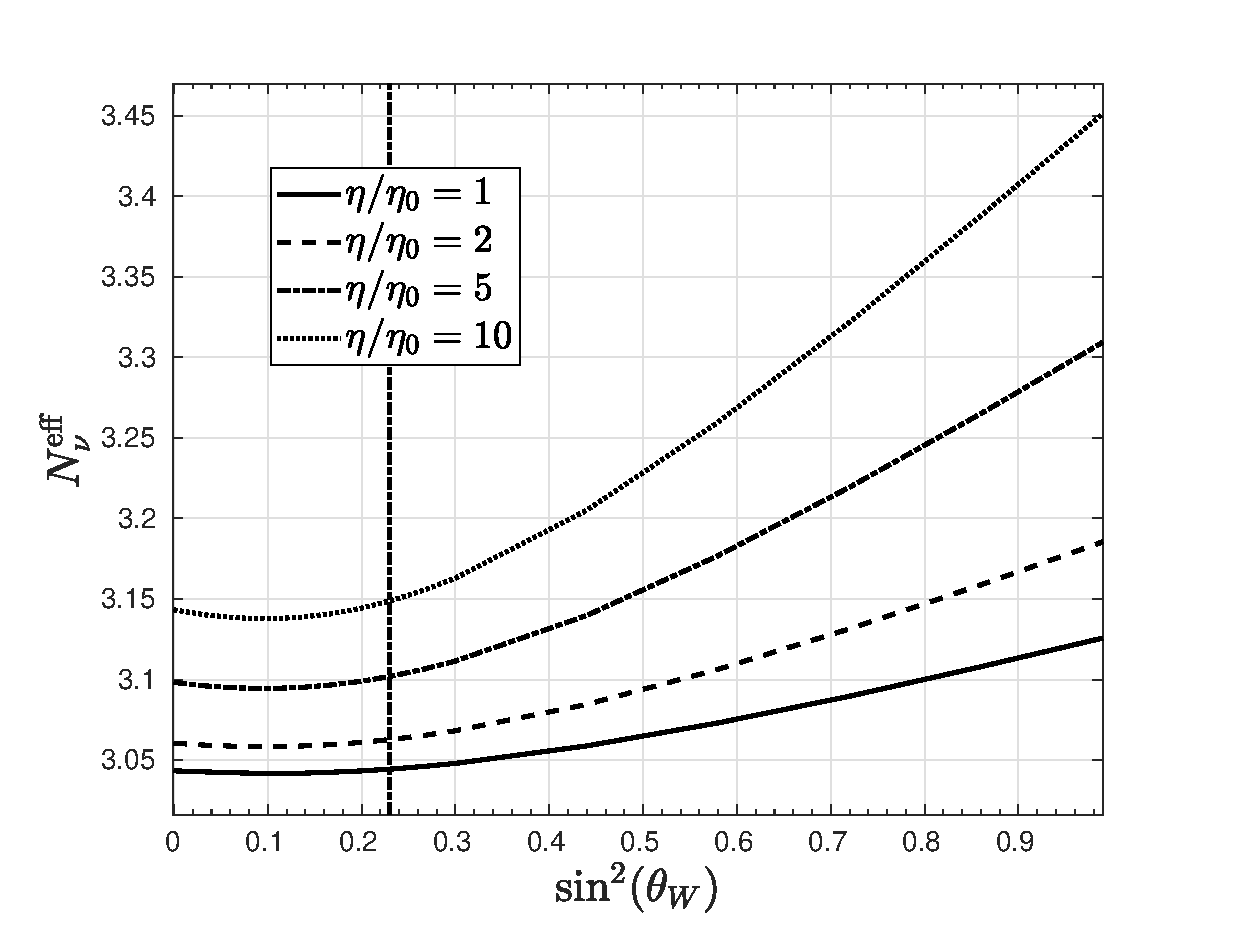
\includegraphics[width=0.70\columnwidth]{04-birrell/ParametricStudies/Figures/N_eff2.eps}
}
\caption{Adapted from \cite{Birrell:2014uka}: Change in effective number of neutrinos  $N_\nu^{\mathrm{eff}}$ as a function of Weinberg angle for  several values of $\eta/\eta_0=1,2,5,10$. Vertical line is $\sin^2(\theta_W)=0.23$.}
\label{N_nu_params}  
 \end{figure}
%%%%%%%%%%%%%%%%%%%%
We performed a least squares fit of $N_\nu^{\mathrm{eff}}$ over the range $0\leq \sin^2(\theta_W)\leq 1$, $1\leq \eta/\eta_0\leq 10$ shown in figure \ref{N_nu_params}, obtaining a result with relative error less than $0.2\%$,
\begin{align}
N_\nu^{\mathrm{eff}}=&3.003-0.095\sin^2(\theta_W) +0.222\sin^4(\theta_W ) -0.164\sin^6(\theta_W )\notag\\
+&\sqrt{\frac{\eta}{\eta_0}}\left(0.043+0.011\sin^2(\theta_W) +0.103\sin^4(\theta_W)\right)\,.
\end{align}
$N_\nu^{\mathrm{eff}}$ is monotonically increasing in $\eta/\eta_0$ with dominant behavior  scaling as $\sqrt{ \eta/\eta_0}$. Monotonicity is to be expected, as increasing $\eta$ decreases the freeze-out temperature and the longer neutrinos are able to remain coupled to $e^\pm$, the more energy and entropy from annihilation is transferred to neutrinos.
%%%%%%%%%%%%%%%%%%%%%%%%%%%%%%%%%%%%%%%
\begin{figure}[ht]
\centerline{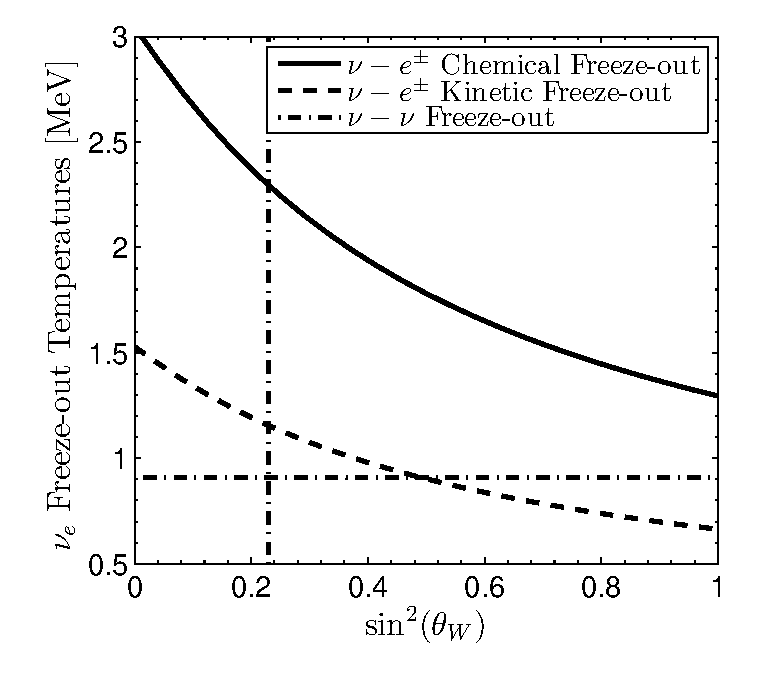
\includegraphics[height=6.3cm]{04-birrell/ParametricStudies/Figures/nu_e_freezeout.eps}\hspace{5mm}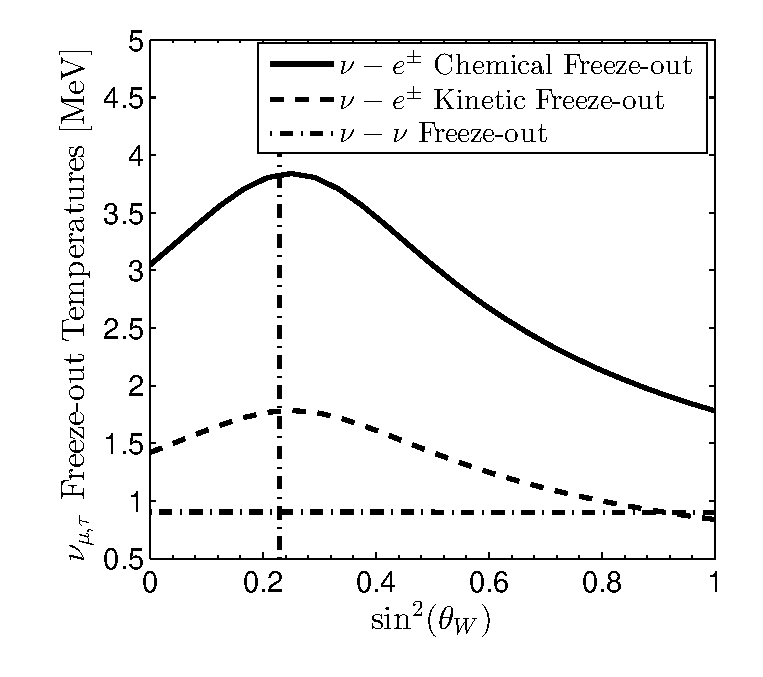
\includegraphics[height=6.3cm]{04-birrell/ParametricStudies/Figures/nu_mu_freezeout.eps}}
\caption{\cccite{Birrell:2014uka}.  Freeze-out temperatures for electron neutrinos (left) and $\mu$, $\tau$ neutrinos (right) for various types of processes, as functions of Weinberg angle. Vertical line is $\sin^2(\theta_W)=0.23$.}\label{fig:freezeoutT_B}
 \end{figure}
%%%%%%%%%%%%%%%%%%%%%%%%%%%%%%%%%%%%%%%
%%%%%%%%%%%%%%%%%%%%%%%%%%%%%%%%%%%%%%%
\begin{figure}[ht]
\centerline{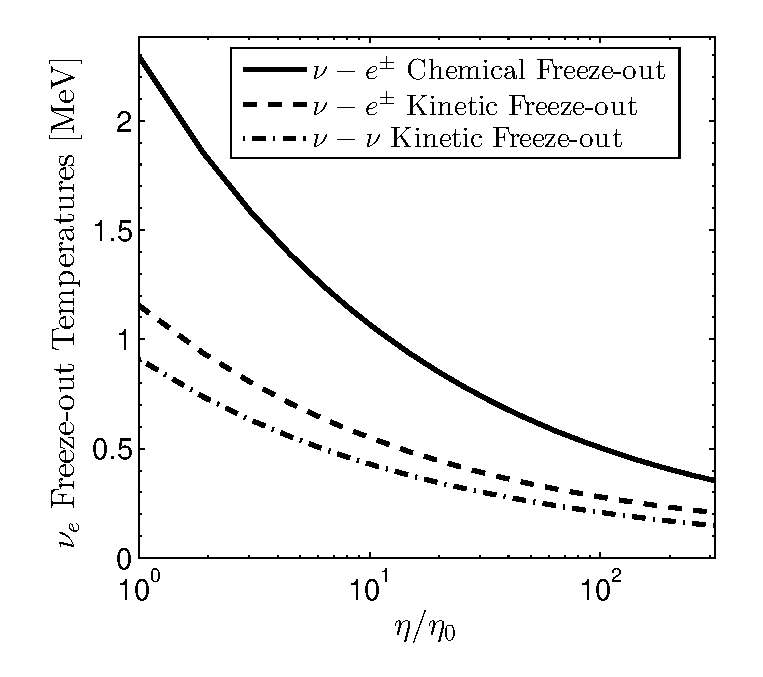
\includegraphics[height=6.3cm]{04-birrell/ParametricStudies/Figures/nu_e_freezeout_GF.eps}\hspace{5mm}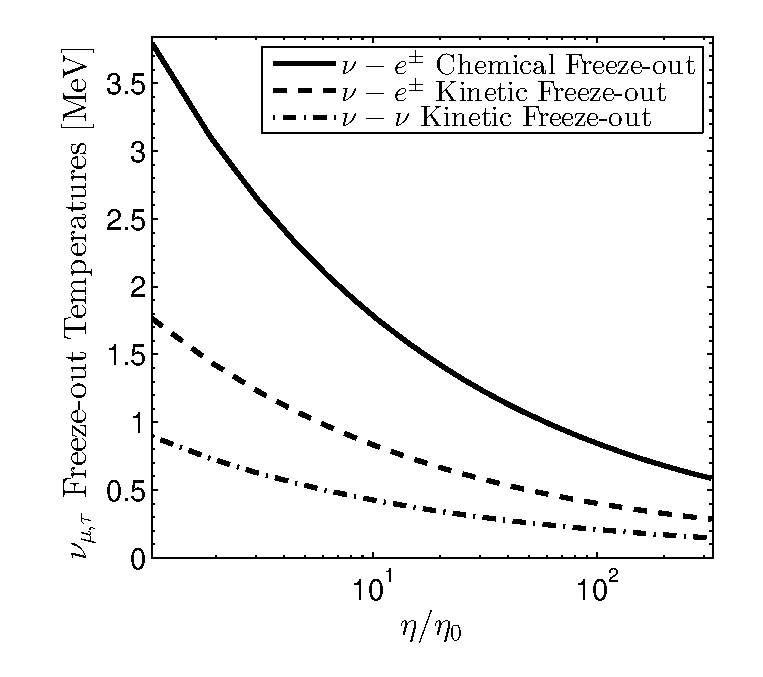
\includegraphics[height=6.3cm]{04-birrell/ParametricStudies/Figures/nu_mu_freezeout_GF.eps}}
\caption{\cccite{Birrell:2014uka}. Freeze-out temperatures for electron neutrinos (left) and $\mu$, $\tau$ neutrinos (right) for various types of processes, as functions of interaction strength.}\label{fig:freezeoutT_eta}
 \end{figure}
%%%%%%%%%%%%%%%%%%%%%%%%%%%%%%%%%%%%%%%



We complement this with fits to the photon to neutrino temperature ratios $ T_\gamma / T_{\nu_e}$, $T_\gamma / T_{\nu_\mu}= T_\gamma / T_{\nu_\tau} $, and the neutrino fugacities, $\Upsilon_{\nu_e}, \Upsilon_{\nu_\mu}=\Upsilon_{\nu_\tau}$, again with relative error less than $0.2\%$,  
\begin{align}
\frac{T_\gamma}{T_{\nu_\mu}}=&1.401+0.015x-0.040x^2+0.029x^3-0.0065y+0.0040xy-0.017x^2y\,, \notag\\
\Upsilon_{\nu_e}=&1.001+0.011x-0.024x^2+0.013x^3-0.005y-0.016xy+0.0006x^2y\,,\notag\\ 
\frac{T_\gamma}{T_{\nu_e}}=&1.401+0.015x-0.034x^2+0.021x^3-0.0066y-0.015xy-0.0045x^2y\,,\notag\\
\Upsilon_{\nu_\mu}=&1.001+0.011x-0.032x^2+0.023x^3-0.0052y+0.0057xy-0.014x^2y\,,
\end{align}
where
\begin{equation}%{align}
x\equiv \sin^2(\theta_W)\, ,\qquad
y\equiv  \sqrt{\frac{\eta}{\eta_0}}\,.
\end{equation}%{align}

%%%%%%%%%%%%%%%%%%%%
\begin{figure}%[ht]
\centerline{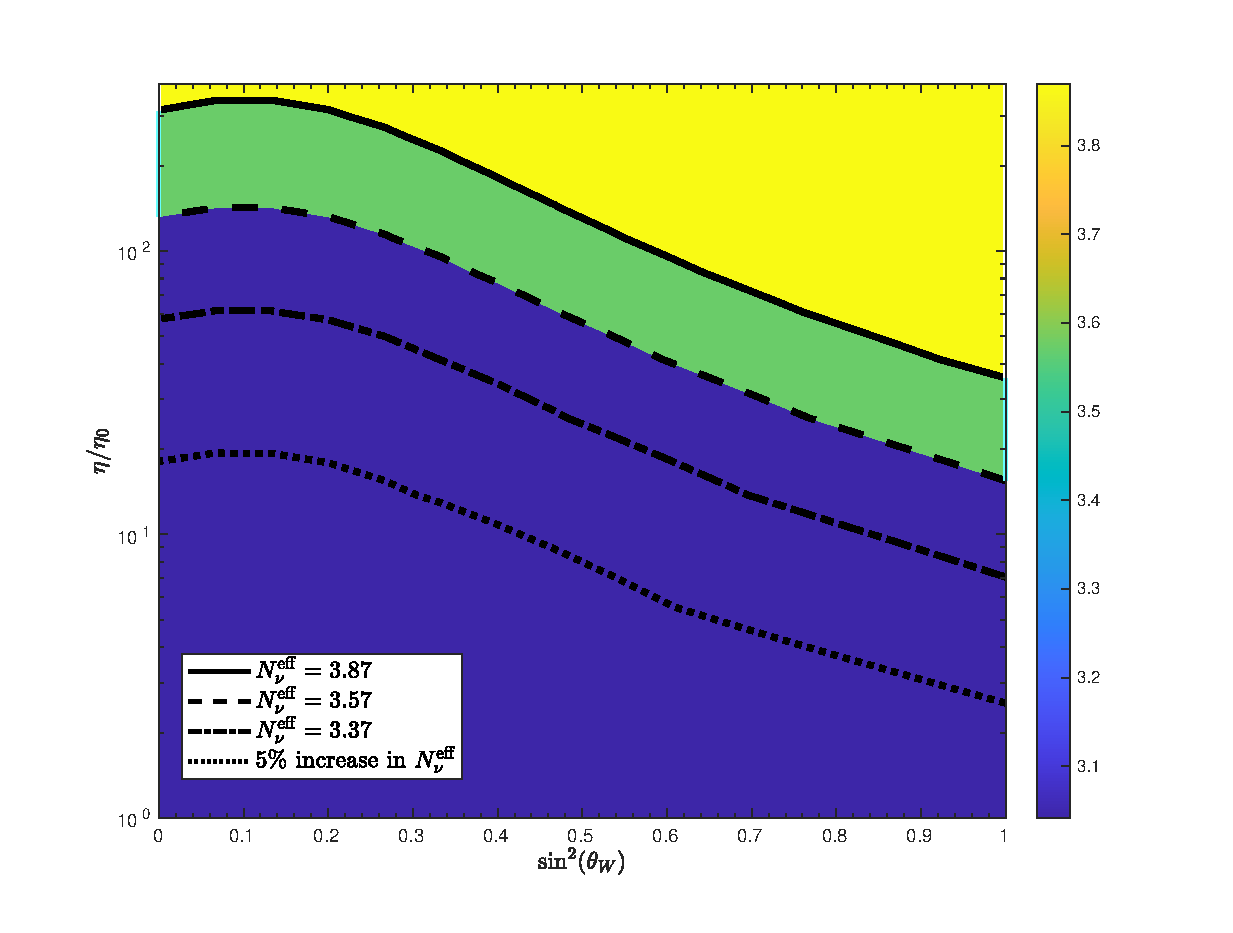
\includegraphics[width=\columnwidth]{04-birrell/ParametricStudies/Figures/region_plot_legend.eps}
}
\caption{Adapted from \cite{Birrell:2014uka}: $N_\nu^{\mathrm{eff}}$ bounds in the $\eta/\eta_0, \sin^2(\theta_W)$ plane. Blue for $N_\nu^{\mathrm{eff}}\in (3.03,3.57)$ corresponding to Ref.~\cite{Planck:2013pxb} CMB+BAO analysis and green extends the region to $N_\nu^{\mathrm{eff}}<3.87$ i.e. to CMB+$H_0$. Dot-dashed line delimits the 1 standard-deviation lower boundary of the second analysis.}
\label{N_nu_domain}
 \end{figure}
%%%%%%%%%%%%%%%%%%%%
The bounds on $N_\nu^{\mathrm{eff}}$ from the Planck analysis \cite{Planck:2013pxb} can be  used to constrain time or temperature variation of $\sin^2(\theta_W)$ and $\eta$.  
In  Figure \ref{N_nu_domain} the blue region shows the combined range of  variation of natural constants  compatible with CMB+BAO and the green region shows  the extension in the range of  variation of  natural constants for CMB+$H_0$, both at a $68\%$ confidence level. The dot-dashed line within the blue region delimits   this latter domain. The dotted line shows the limit of a 5\% change in $N_\nu^{\mathrm{eff}}$.    Any increase in  $\eta/\eta_0$ and/or $\sin^2(\theta_W)$ moves the value of $N_\nu^{\mathrm{eff}}$ into the domain favored by current experimental results.

%%%%%%%%%%%%%%%%%%%%

We have omitted here a discussion of flavor neutrino oscillations. If it weren't for the differences between the matrix elements for the interactions between $e^\pm$ and $\nu_e$ on one hand and $e^\pm$ and $\nu_\mu,\nu_\tau$ on the other, oscillations would have no effect on the flow of entropy into neutrinos and hence no effect on $N_\nu^{\mathrm{eff}}$, but these differences do lead to a modification of $N_\nu^{\mathrm{eff}}$.  In \cite{Mangano:2005cc} the impact of oscillations on neutrino freeze-out for the present day measured values of $\theta_W$ and $\eta$ was investigated.  It was found  that while oscillations redistributed energy amongst the neutrino flavors, the impact on $N_\nu^{\mathrm{eff}}$ was negligible. We have neglected oscillations in our study.



\subsubsection{Primordial Variation of Natural Constants}
We end our study of neutrino freeze-out by exploring what neutrino decoupling in the early Universe can tell us about the values of natural constants when the Universe was about one second old and at an ambient temperature near to 1 MeV (11.6 billion degrees K). Our results were presented assuming that the Universe contains no other effectively massless particles but the three left handed neutrinos and  three corresponding right handed anti-neutrinos. 

In Figure \ref{N_nu_params} we see that, near  the present day value of the Weinberg angle  $\sin^2(\theta_W)\simeq 0.23$, the effect of changing $\sin^2(\theta_W)$ on the decoupling of neutrinos is small. The dominant variance is due to the change  in the coupling strength $\eta/\eta_0$, \req{eta_def}  and \req{eta0_def}. The dotted line in  Figure \ref{N_nu_domain} shows that in order to achieve a change in $N_\nu^{\mathrm{eff}}$ at the level of up to 5\%, i.e., $N_\nu^{\mathrm{eff}}\lesssim 3.2 $,   $\eta/\eta_0$ must change significantly, e.g.,  increasing by an order of magnitude.

We would like to better understand whether, in the primordial Universe, $\eta$ could be significantly (i.e., an order
of magnitude) different from the current value. We explore the rationale governing this
hypothesis by considering the natural constants  contributing to $\eta$ and their required
modification:
\begin{itemize}
\item
In models of emergent gravity we can imagine a `melting' of gravity in the hot primordial
Universe, just like we see the vacuum structure and quark confinement melt. Conversely, and
perhaps more attractive in light of the present day interest in the so called Hubble-tension, there could be
present-era weakening of gravity which would allow the Universe expansion to accelerate and more
generally could also modify the dark energy input into Universe dynamics. Whether such a
variable gravity model can be realized will be a topic for future consideration. Considering
that  $\eta\propto M_p\propto G_N^{-1/2}$ the value of $\eta$ will change in the opposite to the
strength of gravity: An order magnitude change in $\eta$ at the time of neutrino decoupling
translates into two orders of magnitude (inverse) change in the strength of gravity. One would
not think this is a possible scenario but a change in gravity strength by a less extreme factor
could be imagined.
\item
Compared to all other elementary particles the electron mass has an unusually low value. This
could imply a more complicated mass origin of the electron when compared to other elementary
particles which are drawing their mass by the minimal coupling from the Higgs field.  We studied
  a strong field mechanism for electron mass melting recently~\cite{Evans:2019zyk}. Since
$\eta\propto m_e^3$, electron mass would need to change at the time of decoupling of neutrinos by
`only' a factor 2.15 to create an order of magnitude impact on $\eta$.
\item
A modification by `only' a factor of 1.8  in the vacuum  expectation value (VEV) of the Higgs field
$v_0\simeq 246$ GeV  controlling the weak interaction coupling $G_\mathrm{F}\propto 1/v^4$ would
suffice to alter $\eta$ by an order of magnitude. However, if we allow electron mass to be also
Higgs controlled,  three powers of $v$ would cancel and a change in $v$ by an order of magnitude
near to $T\simeq m_e$ would be required. In either case, given our good understanding of the
standard model of particle physics  we do not believe that the  VEV of the Higgs field could be
impacted by the conditions prevailing at the time of neutrino decoupling.
\end{itemize}
To summarize: Gravity is an effective theory poorly understood at a fundamental level. Electron
mass is `anomalously' small and has a scale below the temperature scale of neutrino decoupling.
Thus both could potentially  be the cause of a substantial change in $\eta$. On the other hand the Higgs VEV seems
immutable at neutrino decoupling, considering the relevant scale being 500,000 times greater.

One could argue that time dependence of  $\sin^2(\theta_W)$ remains without a theoretical
motivation, mainly so since in SU(5) model unifying  quarks and leptons a value
$\sin^2(\theta_W)=1/4$  appears. Since this model has been discredited by baryon stability, any
value of $\sin^2(\theta_W)$ seems possible at time of neutrino decoupling, as there is no known
rational for the observed   mixing value of $\sin^2(\theta_W)$.


